\subsection{Sampling diversity and pass@k growth}
\label{sec:results-diversity}

The diversity analysis measures how additional samples change the set of generated candidates. Figure~\ref{fig:diversity-gain} plots answer diversity against pass@k gain. Diffusion models often produce fewer distinct normalized answers and smaller pass@k gains, while the strongest autoregressive high-$k$ models maintain broader output diversity and larger pass@k growth.

\begin{figure}[!htbp]
\centering
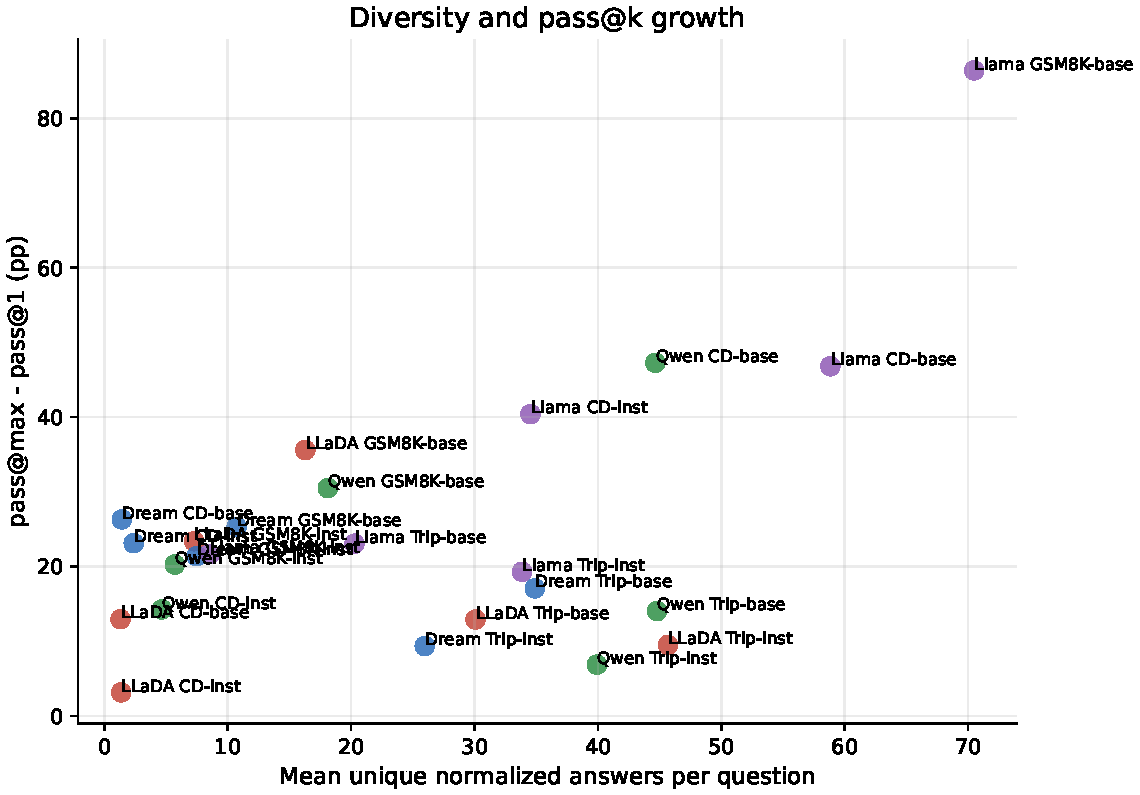
\includegraphics[width=0.84\textwidth]{images/diversity_vs_passk_gain.pdf}
\caption{Mean answer diversity versus pass@k gain across all main comparison conditions. Broader answer diversity tends to accompany larger gains from search on the planning benchmarks.}
\label{fig:diversity-gain}
\end{figure}

\paragraph{Concrete example.} A representative Countdown-cd4 base question with target $39$ and inputs $\{23, 10, 3, 28\}$ illustrates the diversity gap. LLaDA-Base produces one correct normalized chain, \texttt{23+10=33,33/3=11,11+28=39}, in $6$ of its $128$ samples. Qwen-Base produces $94$ distinct first-line candidate chains on the same question, although none is correct for this instance. The example therefore illustrates candidate spread rather than an AR success on that item; across the full $992$-question set, the broader AR spread corresponds to steeper pass@k growth. Additional traces, including paradigm-specific failure cases, are reproduced in Appendix~\ref{sec:appendix-qualitative}.

Countdown base is the clearest case: LLaDA averages only $1.31$ unique normalized answers per question and a $12.93$-point pass@k gain, while Qwen averages $44.65$ unique normalized answers and a $47.27$-point gain. Llama-Base is even broader, with $58.84$ unique normalized answers per question and a $46.80$-point gain. Trip Planning is noisier because parser validity interacts with diversity, but Llama obtains the largest high-$k$ gain in both base and instruct Trip Planning conditions.
